\documentclass[a4paper, 12pt]{article}
\usepackage{geometry}
\geometry{a4paper,
total={170mm,257mm},left=2cm,right=2cm,
top=2cm,bottom=2cm}

\usepackage{color}
\usepackage{hyperref}
\usepackage{mathtext}
\usepackage{amsmath}
\usepackage[utf8]{inputenc}
\usepackage[english,russian]{babel}
\usepackage{graphicx}
\usepackage{float}
\usepackage{tabularx, colortbl}
\usepackage{caption}
\usepackage{textcomp}
\usepackage{multirow}

\begin{document}
\title{\textbf{Отчёт о выполнении лабораторной работы 1.1.4.}}
\author{Рачков Михаил Васильевич Б01-201}
\date{13.09.2022}
\maketitle
\begin{center}
\rule{135mm}{1pt}
\end{center}

\section*{Измерение интенсивности \\ радиационного фона}

\subsection*{Цель работы}
Применение методов обработки экспериментальных данных для изучения статистических закономерностей при измерении интенсивности радиоактивного фона.

\subsection*{Оборудование}
Счётчик Гейгера-Мюллера (СТС-6), блок питания. компьютер.

\subsection*{Теоретическая справка}

Среднеквадратичная ошибка числа отчетов, измеренного за некоторый интервал времени равна:

\begin{equation} \label{eq:1}
    \sigma = \sqrt{n}
\end{equation}

Тогда результат измерения запишется так:

\begin{equation} \label{eq:2}
    n_0 = n \pm \sqrt{n}
\end{equation}

При $N$ измерениях среднее значение числа посчитанных за одно измерение частиц может быть посчитано по формуле:

\begin{equation} \label{eq:3}
    \bar{n} = \frac{1}{N} \sum_{i=1}^N {n_i}
\end{equation}

А стандартная ошибка отдельного измерения может быть оценена по формуле:

\begin{equation} \label{eq:4}
    \sigma_{отд} = \sqrt {\frac{1}{N} \sum_{i=1}^N ({n_i - \bar{n}})^2}
\end{equation}

В соответствии с формулой \eqref{eq:1} следует ожидать, что это ошибка будет близка к $\sqrt{n_i}$.  Поскольку $n_i$ различны, мы будем получать различные оценки для $\sigma_{отд}$. Какие-то из них будут лучше, какие-то -- хуже. Ближе всего к значению $\sigma_{отд}$ будет корень из усредненного измерения, т.е.

\begin{equation} \label{eq:5}
    \sigma_{отд} \approx \sqrt{\bar{n}}
\end{equation}

Величина $\bar{n}$ из формулы \eqref{eq:3} тоже является случайной, ее отклонение от истинного значения может быть определено по формуле:

\begin{equation} \label{eq:6}
    \sigma_{\bar{n}} = \frac{1}{N} \sqrt {\sum_{i=1}^N ({n_i - \bar{n}})^2} = \frac {\sigma_{отд}}{\sqrt {N}}
\end{equation}

Обычно наибольший интерес представляет относительная погрешность. Для рассмотрения серии из $N$ экспериментов по 20 с. относительная ошибка отдельного измерения (т.е. ожидаемое отличие $n_i$ от $n_0$) равна:

\begin{equation} \label{eq:7}
   \varepsilon_{отд} = \frac {\sigma_{отд}}{n_i} \approx \frac {1}{\sqrt {n_i}}
\end{equation}

Аналогичным образом определяется относительная ошибка в определении среднего по всем измерениям значения $\bar{n}$.

\begin{equation} \label{eq:8}
    \varepsilon_{\bar{n}} = \frac {\sigma_{\bar{n}}}{\bar{n}} = \frac {\sigma_{отд}}{\bar{n} \sqrt {N}} \approx \frac {1}{\sqrt {\bar {n} N}}
\end{equation}

\subsection*{Ход работы}
\begin{enumerate}

    \item Включаем компьютер. (Запускается измерение данных для демонстрационного эксперимента)
    \item В результате демонстрационного эксперимента убеждаемся, что при увеличении числа измерений:

        \begin{enumerate}
            \item измеряемая величина флуктуирует;
            \item флуктуации среднего значения измеряемой величины уменьшаются, и с ростом количества измерений среднее значение выходит на постоянную величину;
            \item флуктуации величины погрешности отдельного измерения уменьшаются, и с ростом количества измерений погрешность отдельного измерения (погрешность метода) выходит на постоянную величину
            \item флуктуации величины погрешности среднего значения уменьшаются, а сама величина убывает.
        \end{enumerate}

    \item Переходим к основному эксперименту: измерение плотности потока космического излучения за 20 с. На компьютере проведем обработку, аналогичную сделанной в демонстрационном эксперименте. Результаты приведем в таблицы \ref{tabl:data_raw_20} и \ref{tabl:data_hist_10}. Примечание: таблица \ref{tabl:data_raw_20} устроена так, что, например, результат 123-го опыта лежит на пересечении строки, обозначенной 120 и столбца с номером 3.

    \begin{table}[h!]
        \centering
        \begin{tabular}{| c || c | c | c | c | c | c | c | c | c | c |}
        \hline
        \textnumero~{опыта} & \textbf{1}  & \textbf{2}  & \textbf{3}  & \textbf{4}  & \textbf{5}  & \textbf{6}  & \textbf{7}  & \textbf{8}  & \textbf{9}  & \textbf{110}\\\hline\hline
        \textbf{0}   & 21 & 21 & 24 & 32 & 26 & 19 & 33 & 25 & 19 & 24 \\\hline
        \textbf{10}  & 29 & 24 & 28 & 30 & 28 & 24 & 31 & 23 & 27 & 24 \\\hline
        \textbf{20}  & 26 & 16 & 18 & 22 & 32 & 22 & 18 & 30 & 25 & 24 \\\hline
        \textbf{30}  & 24 & 28 & 21 & 17 & 22 & 25 & 27 & 18 & 26 & 30 \\\hline
        \textbf{40}  & 24 & 21 & 26 & 24 & 19 & 26 & 35 & 33 & 20 & 22 \\\hline
        \textbf{50}  & 27 & 23 & 30 & 27 & 32 & 20 & 24 & 31 & 13 & 22 \\\hline
        \textbf{60}  & 16 & 30 & 23 & 23 & 23 & 22 & 23 & 25 & 29 & 32 \\\hline
        \textbf{70}  & 30 & 24 & 25 & 23 & 24 & 29 & 19 & 22 & 15 & 18 \\\hline
        \textbf{80} & 24 & 21 & 14 & 25 & 24 & 29 & 24 & 34 & 26 & 20 \\\hline
        \textbf{90} & 21 & 28 & 22 & 43 & 29 & 19 & 22 & 21 & 25 & 22 \\\hline
        \textbf{100} & 26 & 24 & 30 & 22 & 40 & 22 & 28 & 25 & 20 & 28 \\\hline
        \textbf{110} & 22 & 22 & 28 & 27 & 22 & 27 & 35 & 20 & 24 & 22 \\\hline
        \textbf{120} & 23 & 22 & 29 & 30 & 32 & 39 & 27 & 20 & 21 & 36 \\\hline
        \textbf{130} & 16 & 27 & 30 & 22 & 25 & 22 & 27 & 20 & 29 & 15 \\\hline
        \textbf{140} & 25 & 20 & 35 & 20 & 28 & 34 & 23 & 22 & 22 & 22 \\\hline
        \textbf{150} & 28 & 17 & 26 & 27 & 19 & 19 & 26 & 24 & 23 & 24 \\\hline
        \textbf{160} & 14 & 26 & 18 & 28 & 32 & 26 & 19 & 32 & 27 & 18 \\\hline
        \textbf{170} & 28 & 19 & 22 & 21 & 17 & 22 & 24 & 26 & 25 & 25 \\\hline
        \textbf{180} & 32 & 25 & 20 & 23 & 26 & 31 & 28 & 31 & 24 & 32 \\\hline
        \textbf{190} & 28 & 29 & 20 & 15 & 27 & 20 & 19 & 24 & 23 & 28 \\\hline
        \end{tabular}
        \caption{Число срабатываний счетчика за 20 секунд}
        \label{tabl:data_raw_20}
    \end{table}

    \item Разобьем результаты из таблицы \ref{tabl:data_raw_20} в порядке их получения на группы по 2 и сложим числа в каждой группе. Это будет соответствовать $N_2=100$ измерениям по 40 c каждое. Резльтаты сведем в таблицу \ref{tabl:data_raw_40}

    \begin{table}[h!]
        \centering
        \begin{tabular}{| c | c | c |}
        \hline
        \textbf{Число импульсов $n_i$} & \textbf{Число случаев} & \textbf{Доля случаев $w_n$} \\\hline\hline
        4                        & 1                      & 0.0025                \\\hline
        5                        & 3                      & 0.0075                \\\hline
        6                        & 7                      & 0.0175                \\\hline
        7                        & 26                     & 0.0650                \\\hline
        8                        & 29                     & 0.0725                \\\hline
        9                        & 22                     & 0.0550                \\\hline
        10                       & 35                     & 0.0875                \\\hline
        11                       & 52                     & 0.1300                \\\hline
        12                       & 42                     & 0.1050                \\\hline
        13                       & 38                     & 0.0950                \\\hline
        14                       & 38                     & 0.0950                \\\hline
        15                       & 27                     & 0.0675                \\\hline
        16                       & 27                     & 0.0675                \\\hline
        17                       & 21                     & 0.0525                \\\hline
        18                       & 16                     & 0.0400                \\\hline
        19                       & 5                      & 0.0125                \\\hline
        20                       & 5                      & 0.0125                \\\hline
        21                       & 2                      & 0.0050                \\\hline
        22                       & 2                      & 0.0050                \\\hline
        23                       & 2                      & 0.0050                \\\hline
        \end{tabular}
        \caption{Данные для построения гистограммы распределения числа срабатываний счетчика за 10 с.}
        \label{tabl:data_hist_10}
    \end{table}

    \begin{table}[h!]
        \centering
        \begin{tabular}{|c || c | c | c | c | c | c | c | c | c | c |}
        \hline
        \textnumero~{опыта}   & \textbf{1} & \textbf{2} & \textbf{3} & \textbf{4} & \textbf{5} & \textbf{6} & \textbf{7} & \textbf{8} & \textbf{9} & \textbf{10} \\ \hline\hline
        \textbf{0}  & 42         & 56         & 45         & 58         & 43         & 53         & 58         & 52         & 54         & 51          \\ \hline
        \textbf{10} & 42         & 40         & 54         & 48         & 49         & 52         & 38         & 47         & 45         & 56          \\ \hline
        \textbf{20} & 45         & 50         & 45         & 68         & 42         & 50         & 57         & 52         & 55         & 35          \\ \hline
        \textbf{30} & 46         & 46         & 45         & 48         & 61         & 54         & 48         & 53         & 41         & 33          \\ \hline
        \textbf{40} & 45         & 39         & 53         & 58         & 46         & 49         & 65         & 48         & 43         & 47          \\ \hline
        \textbf{50} & 50         & 52         & 62         & 53         & 48         & 44         & 55         & 49         & 55         & 46          \\ \hline
        \textbf{60} & 45         & 59         & 71         & 47         & 57         & 43         & 52         & 47         & 47         & 44          \\ \hline
        \textbf{70} & 45         & 55         & 62         & 45         & 44         & 45         & 53         & 38         & 50         & 47          \\ \hline
        \textbf{80} & 40         & 46         & 58         & 51         & 45         & 47         & 43         & 39         & 50         & 50          \\ \hline
        \textbf{90} & 57         & 43         & 57         & 59         & 56         & 57         & 35         & 47         & 43         & 51          \\ \hline
        \end{tabular}
        \caption{Число срабатываний счетчика за 40 с.}
        \label{tabl:data_raw_40}
    \end{table}


    \item Представим результаты из таблицы \ref{tabl:data_raw_40} в виде, удобном для построения гистограммы. Результаты занесем в таблицу \ref{tabl:data_hist_40}. Гистограммы распределений среднего числа отсчетов за 10 и 40 с. строим на одном графике (рис \ref{pic:hists}). При этом для второй гистограммы увеличиваем шкалу деления оси абсцисс в 4 раза, чтобы максимумы гистограмм совпали.
    \begin{table}[h!]
        \centering
        \begin{tabular}{| c | c | c |}
        \hline
        \textbf{Число импульсов $n_i$} & \textbf{Число случаев} & \textbf{Доля случаев $w_n$} \\\hline\hline
        33 & 1  & 0.005 \\\hline
        34 & 0  & 0     \\\hline
        35 & 2  & 0.010  \\\hline
        36 & 0  & 0     \\\hline
        37 & 0  & 0     \\\hline
        38 & 2  & 0.010  \\\hline
        39 & 2  & 0.010  \\\hline
        40 & 2  & 0.010  \\\hline
        41 & 1  & 0.005 \\\hline
        42 & 3  & 0.015 \\\hline
        43 & 6  & 0.030  \\\hline
        44 & 3  & 0.015 \\\hline
        45 & 11 & 0.055 \\\hline
        46 & 5  & 0.025 \\\hline
        47 & 8  & 0.040  \\\hline
        48 & 5  & 0.025 \\\hline
        49 & 3  & 0.015 \\\hline
        50 & 6  & 0.030  \\\hline
        51 & 3  & 0.015 \\\hline
        52 & 5  & 0.025 \\\hline
        53 & 5  & 0.025 \\\hline
        54 & 3  & 0.015 \\\hline
        55 & 4  & 0.020  \\\hline
        56 & 3  & 0.015 \\\hline
        57 & 5  & 0.025 \\\hline
        58 & 4  & 0.020  \\\hline
        59 & 2  & 0.010  \\\hline
        60 & 0  & 0     \\\hline
        61 & 1  & 0.005 \\\hline
        62 & 2  & 0.010  \\\hline
        63 & 0  & 0     \\\hline
        64 & 0  & 0     \\\hline
        65 & 1  & 0.005 \\\hline
        66 & 0  & 0     \\\hline
        67 & 0  & 0     \\\hline
        68 & 1  & 0.005 \\\hline
        69 & 0  & 0     \\\hline
        70 & 0  & 0     \\\hline
        71 & 1  & 0.005 \\\hline
        39 & 1  & 0.005 \\\hline
        \end{tabular}
        \caption{Данные для построения гистограммы распределения числа срабатываний счетчика за 40 с.}
        \label{tabl:data_hist_40}
    \end{table}

    \begin{figure}[h!]
        \centering
        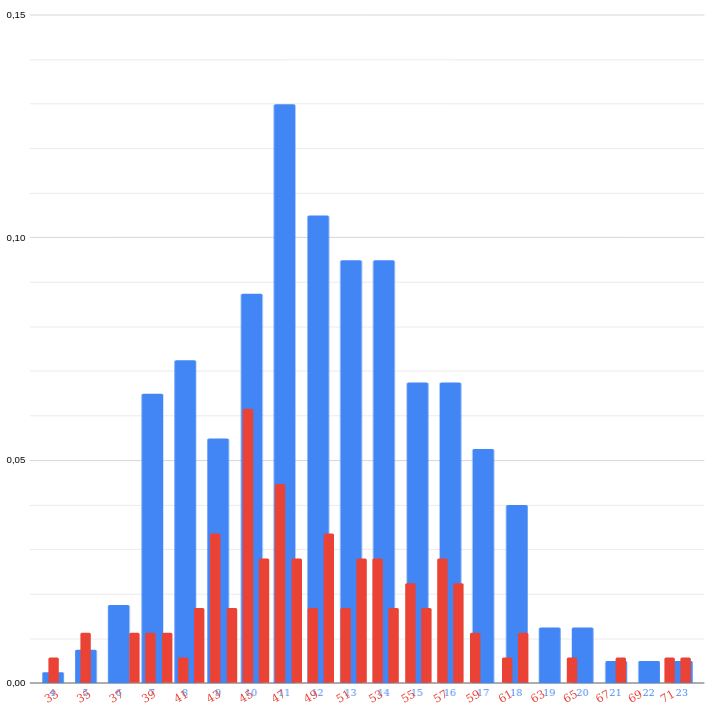
\includegraphics[width=10cm]{hist.1.1.4.png}
        \caption{Гистограмма для $\textcolor{blue}{\tau = 10~c~}$и $\textcolor{red}{\tau = 40~c}$}
        \label{pic:hists}
    \end{figure}

    Используя формулу \ref{eq:3}, определим среднее значение срабатывания счетчика за 10  и 40 с. соответственно:
\[
    \bar{n}_{10} = \frac{1}{N_1} \sum_{i=1}^{N_{1}} {n_i} = \frac{4934}{400} = 12.335
\]

\[
    \bar{n}_{40} = \frac{1}{N_2} \sum_{i=1}^{N_{2}} {n_i} = \frac{4934}{100} = 49.34
\]

 Найдем среднеквадратичную ошибку отдельного измерения (для 10 с подсчитывается автоматически) по формуле \eqref{eq:4}
\[
    \sigma_{отд_{10}} = \sqrt {\frac{1}{N_1} \sum_{i=1}^{N_{1}} ({n_i - \bar{n}})^2} = 3.5601
\]

\[
    \sigma_{отд_{40}} = \sqrt {\frac{1}{N_2} \sum_{i=1}^{N_{2}} ({n_i - \bar{n}})^2} = 7.0342
\]

 Убедимся в верности формулы \eqref{eq:5}. Действительно:
\[
    \sigma_{отд_{10}} = 3.5601 \approx \sqrt{12.335} = 3.5121
\]

\[
    \sigma_{отд_{40}} = 7.0342 \approx \sqrt{49.34} = 7.0242
\]

 Определим долю случаев, когда отклонение от среднего значения не превышают $\sigma_{отд}$ и $2\sigma_{отд}$ и занесем результат в таблицу \ref{tabl:percent_errors}.

\begin{table}[!h]
    \centering
    \begin{tabular}{|c|c|c|c|c|}
        \hline
         & Ошибка & Число случаев & Доля случаев, \% & Теоретическая оценка \\ \hline
        \multirow{2}{*}{Для $\tau = 10~c.$} & $\pm \sigma_{отд_{10}}$ & 259 & 64.75 & 68 \\ \cline{2-5}
        & $\pm 2 \sigma_{отд_{10}}$ & 385 & 96.25 & 95 \\ \hline
        \multirow{2}{*}{Для $\tau = 40~c.$} &$ \pm \sigma_{отд_{40}}$ & 69 & 69 & 68 \\ \cline{2-5}
        & $\pm 2 \sigma_{отд_{40}}$ & 93 & 93 & 95 \\ \hline
    \end{tabular}
    \caption{Сравнение доли значений внутри интервалов с теоретическими значениями}
    \label{tabl:percent_errors}
\end{table}

 Сравним среднеквадратичные ошибки отдельных измерений для двух распределений: $\bar{n}_{10} = 12.335$;  $\sigma_{отд_{10}} = 3.5601$;  $\bar{n}_{40} = 49.34$;  $\sigma_{отд_{40}} = 7.0342$. Отсюда видно, что хоть $\sigma_{отд_{40}} > \sigma_{отд_{10}}$, полуширина второго распределения меньше:
\[
    \frac{\sigma_{отд_{10}}}{\bar{n}_{10}} \approx 28.86\% > \frac{\sigma_{отд_{40}}}{\bar{n}_{40}} \approx 14.26\%
\]

Кстати, тот же вывод можно сделать, посмотрев на гистограммы на рисунке \ref{pic:hists}.

 Определмим стандартную ошибку величин  $\bar{n}_{10}$ и $\bar{n}_{40}$ и относительную ошибку тех же величин для $N_1 = 400$ и $N_2 = 100$ соответственно. По формуле \eqref{eq:6}:
\[
    \sigma_{\bar{n}_{10}} = \frac{\sigma_{отд_{10}}}{\sqrt{N_1}} \approx 0.178
\]

Аналогично для $\bar{n}_{40}$
\[
    \sigma_{\bar{n}_{40}} = \frac{\sigma_{отд_{40}}}{\sqrt{N_2}} \approx 0.703
\]

Найдем относительную ошибку по первому равенству \eqref{eq:8}

Для $\bar{n}_{10}$:
\[
    \varepsilon_{\bar{n}_{10}} = \frac{\sigma_{\bar{n}_{10}}}{\bar{n}_{10}} \cdot 100\% \approx 1.443\%
\]

И аналогично для $\bar{n}_{40}$:
\[
    \varepsilon_{\bar{n}_{40}} = \frac{\sigma_{\bar{n}_{40}}}{\bar{n}_{40}} \cdot 100\% \approx 1.425\%
\]

 Окончательный результат:
\[
    n_{\tau=10c.} = \bar{n}_{10} \pm \sigma_{\bar{n}_{10}} = 12.335 \pm 0.178 ~ (частиц)
\]

\[
    n_{\tau=40c.} = \bar{n}_{40} \pm \sigma_{\bar{n}_{40}} = 49.34 \pm 0.71 ~ (частиц)
\]

\item  \textbf{Заключение.}
В работе были построены гистограммы распределения числа отсчетов за 10 и 40 с. соответственно, найдены относительные и абсолютные погрешности вычислений, определен итоговый результат: среднее количество частиц за 10 и 40 с., а также количество и процент измерений, находящихся в $\sigma$-- и $2\sigma$-- интервалах относительно среднего значения. Все это позволило продемонстрировать навыки математической обработки полученных данных.


\end{enumerate}

\end{document}



